%----------------------------------------------------------------------------------------
%	PACKAGES AND DOCUMENT CONFIGURATIONS
%----------------------------------------------------------------------------------------
\documentclass[11pt]{article}
\usepackage{amsmath} % Required for some math elements
\usepackage[usenames,dvipsnames]{xcolor}
\usepackage{lipsum} 
\usepackage{cite}
\usepackage{graphicx} % Required for the inclusion of images
\usepackage{algorithmic}
\usepackage{array}
\usepackage{bookmark}
\usepackage{listings}
\usepackage{amssymb}
\usepackage{enumitem}
\usepackage[margin=24mm]{geometry}
\usepackage[caption=false, font=footnotesize]{subfig}
\usepackage{multirow}
\usepackage[active,tightpage]{preview}
\usepackage{hyperref} 

\renewcommand{\PreviewBorder}{1in}
\newcommand{\Newpage}{\end{preview}\begin{preview}}

\newlist{steps}{enumerate}{1}
\setlist[steps, 1]{label = Step \arabic*:}

\hypersetup{ %color attributes of citation, link, etc.
    colorlinks=true,
    linkcolor=blue,
    filecolor=gray,      
    urlcolor=blue,
    citecolor=blue,
}

 
\lstdefinelanguage{VHDL}{
    morekeywords=[1]{
        library,use,all,entity,is,port,in,out,end,architecture,of,begin,and,or,Not,downto,ALL
    },
    morekeywords=[2]{
        STD_LOGIC_VECTOR,STD_LOGIC,IEEE,STD_LOGIC_1164,NUMERIC_STD,STD_LOGIC_ARITH,STD_LOGIC_UNSIGNED,std_logic_vector,std_logic
    },
    morecomment=[l]--
}

\definecolor{keyword}{rgb}{0,0.3,0.7}
\definecolor{STD}{rgb}{0.9,0.0,0.7}
\definecolor{comment}{rgb}{0.0,0.6,0.1}

\lstdefinestyle{vhdl}{
   language     = VHDL,
   basicstyle   = \footnotesize\ttfamily,
   keywordstyle = [1]\color{keyword}\bfseries,
   keywordstyle = [2]\color{STD}\bfseries,
   commentstyle = \color{comment}
   breaklines=true,                % sets automatic line breaking
   tabsize=3		                   % sets default tabsize to 2 spaces
}


\newcommand{\matlab}{\textsc{Matlab }} %very important and totally necessary addition

\newcommand\Item[1][]{%
    \ifx\relax#1\relax  \item \else \item[#1] \fi
    \abovedisplayskip=0pt\abovedisplayshortskip=0pt~\vspace*{-\baselineskip}}
%----------------------------------------------------------------------------------------
%	DOCUMENT INFORMATION
%----------------------------------------------------------------------------------------
 
\title{ECEN302 : Integrated Digital Electronics \\ Assignment 2 Submission}
\author{Daniel Eisen : 300447549}
\date{\today}

\begin{document}
\begin{preview}
\maketitle
%----------------------------------------------------------------------------------------
%	DOCUMENT CONTENT
%----------------------------------------------------------------------------------------
\begin{enumerate}
    \item \textit{\textbf{List three advantages of scaling down the feature sizes of silicon devices.}}
    
    \begin{itemize}
        \item Higher density means more transistors on a single device
        \item Smaller distance means faster propagation tome and lower power loss.
        \item Smaller sized dies can be run faster and cooler 
    \end{itemize}
    
    \item \textit{\textbf{List two consequences of scaling down the feature sizes of silicon devices.}}
    
    \begin{itemize}
        \item As feature sizes decrease the sum effect of slow atomic diffusion through the semiconductor material decrease the time until the device is unusable.
        \item At smaller and smaller "trace" sizes the risk/probability of electrons quantum tunnelling becomes significant.  
    \end{itemize}
    
    \item \textit{\textbf{Briefly discuss and compare the performance and typical uses of microprocessors and FPGAs.}}
    
    Microprocessors and FPGAs differ in complexity, designing for and in traditional deployment.
    Microprocessors have a fixed instruction set, hardwired logic blocks and executes instructions sequentially per cycle; they can run very fast at sequential task and are the typical use for tradition computing, cpu's etc.
    
    An FPGA doesn’t have any hardwired logic blocks and consist of logic blocks laid out like a net with each junction containing a switch that the user program. This determines how the logic of each block is determined. For these reasons a traditional use case for FPGA is to configure them for large, high performant parallel processing tasks. While they may run are lower clock speeds than top shelf microprocessors the ability to process large amounts to independent parallel data per cycle has made them invaluable in image/video processing, ML/AI, and signal processing. 
    
    
    \item \textit{\textbf{List four advantages of integrating a microprocessor and an FPGA onto a single chip.}}
    
    \begin{itemize}
        \item Able deploy a more traditional sequential CPU based workload that can make use of parallel hardware accelerated processing.
        \item Same die mean higher bandwidth communication between the to devices.
        \item More efficient power usage due to single die.
        \item Reduce requirement of auxiliary interfacing components.
    \end{itemize}
    
    \item \textit{\textbf{Provide one application or product example that benefits from having both a microprocessor and a FPGA.}}
    
    High speed portable digital oscilloscope, such as the DS213. This used a ARM cortex m3 for the general purpose processing and operation and an FPGA to manage/drive the large amount of data from the inputs ADCs.

    \item \textit{\textbf{In a RF receiver signal chain, why is it advantageous to have the ADC as close as possible to the Antenna?}}
    
    Reduce analog signal line length as much as possible to reduce interference from noise and reactive coupling, as to digital output signals are much harder to corrupt.

    \item \textit{\textbf{Describe the operation of the OSERDES and ISERDES FPGA I/O blocks.}}
    OSERDES ((Output parallel to serial converter) and ISERDES (Input serial to parallel converter) are the IO interface responsible for converting between individually slower internal parallel data lines to a much higher speed exterior serial data stream. 
    

    \item \textit{\textbf{Describe, with the aid of diagrams, how you would connect the AD9739 DAC to a Xilinx 7 series device and run the DAC at 2GSPS (note: you do not need to create a detailed schematic diagram).}}
    By using 8 DDS's and sending two LVDS data streams with the clocking shown below, the AD9739 can be sampled at 2Ghz. 


    \begin{center}
        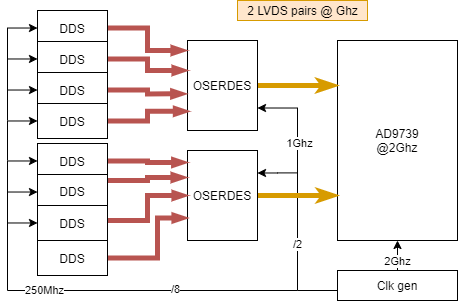
\includegraphics[width=0.75\textwidth]{res/afsdffg.png}
    \end{center}
    

\end{enumerate}

\end{preview}
\end{document}  